
\documentclass[11pt]{article}
\usepackage{tikz}
\usetikzlibrary{shapes, arrows}
\usepackage[hmargin=1in,vmargin=1in]{geometry}
\usepackage{xcolor}
\usepackage{enumitem} 
\usepackage{wrapfig}
\usepackage{amsmath,amssymb,amsfonts,url,sectsty,framed,tcolorbox,framed}
\newcommand{\pf}{{\bf Proof: }}
\newtheorem{theorem}{Theorem}
\newtheorem{lemma}{Lemma}
\newtheorem{proposition}{Proposition}
\newtheorem{definition}{Definition}  
\newtheorem{remark}{Remark}
\newcommand{\qed}{\hfill \rule{2mm}{2mm}}


\begin{document}
	%%%%%%%%%%%%%%%%%%%%%%%%%%%%%%%%%%%%%%%%%%%%%%%%%%%%%%%%%%%%%%%%%%%%%
	\noindent
	\rule{\textwidth}{1pt}
	\begin{center}
		{\bf [CS304] Introduction to Cryptography and Network Security}
	\end{center}
	Course Instructor: Dr. Dibyendu Roy \hfill Winter 2022-2023\\
	Scribed by : Pallikonda Sai Teja  \hfill Lecture (Week 01)\\
	Student ID:202011052\\
	\rule{\textwidth}{1pt}
	
	\section{Introduction}
	
	\begin{itemize}
		\item Cryptography:The part where we develop algorithms to get security / Designing the algorithm.
		\item Cryptanalysis: It is  to break the security of a designed algorithm.
	\end{itemize}
	Cryptology = Cryptography + Cryptanalysis.\\
	NIST standardizes cryptographic algorithms\\
	\section{Encryption and Decryption }
	$\Rightarrow$ Encryption:The process of converting plaintext into Ciphertext .
	
	\begin{center}
		$E(P,k) = C$
	\end{center}
	Plain Text + Secret Key = Cipher Text. \\
	$\Rightarrow$ Decryption:The process of converting Ciphertext into  plaintext. \newline
	\begin{center}
		$D(C,k) = P$
	\end{center}
	
	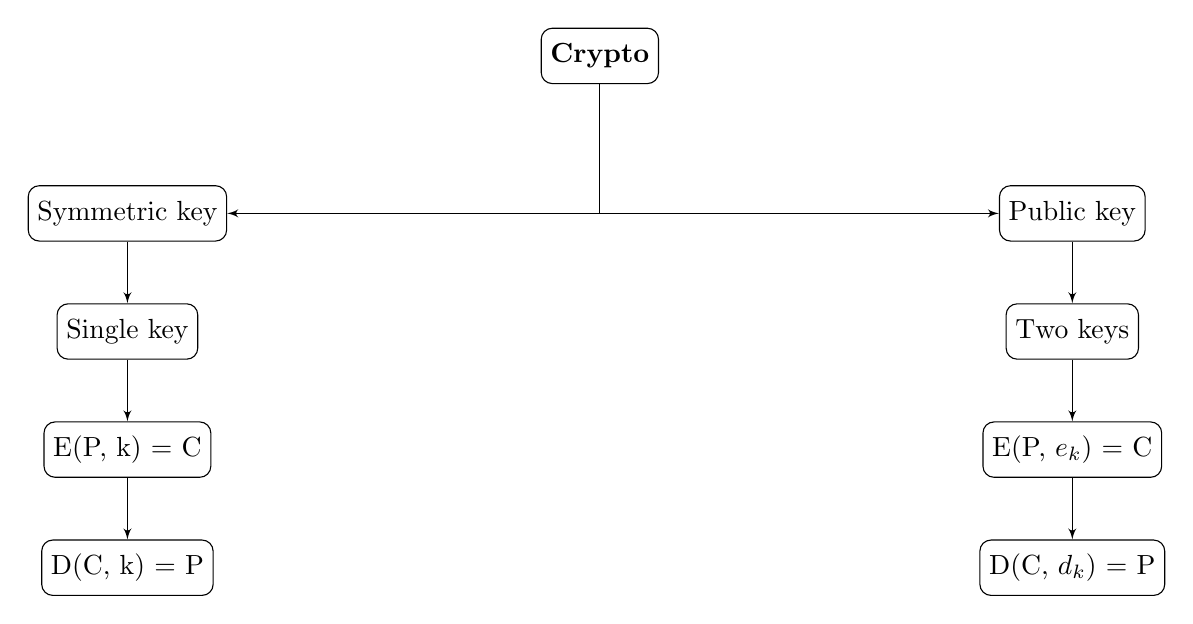
\begin{tikzpicture}
		\tikzstyle{terminator} = [rectangle, draw, text centered, rounded corners, minimum height=2em]
		\tikzstyle{connector} = [draw, -latex']
		\node [terminator] at (0,0) (start) {\textbf{Crypto}};
		\node [terminator] at (-6,-2) (data10) {Symmetric key};
		\node [terminator] at (-6,-3.5) (data11) {Single key};
		\node [terminator] at (-6,-5) (data12) {E(P, k) = C};
		\node [terminator] at (-6,-6.5) (data13) {D(C, k) = P};
		\node [terminator] at (6,-2) (data20) {Public key};
		\node [terminator] at (6,-3.5) (data21) {Two keys};
		\node [terminator] at (6,-5) (data22) {E(P, $e_k$) = C};
		\node [terminator] at (6,-6.5) (data23) {D(C, $d_k$) = P};
		\path [connector] (start) |- (data10);
		\path [connector] (start) |- (data20);
		\path [connector] (data10) -- (data11);
		\path [connector] (data11) -- (data12);
		\path [connector] (data12) -- (data13);
		\path [connector] (data20) -- (data21);
		\path [connector] (data21) -- (data22);
		\path [connector] (data22) -- (data23);
	\end{tikzpicture}
	
	
	\section{Security Services in Cryptograpy}
	\begin{enumerate}
		\item Confidentiality:Ensuring that no one can read the message except the intended receiver .
		\item Integrity: Assuring the receiver that the received message has not been altered in any way from the original.
		\item Authentication: verification of one's identity.
		\item Non-repudiation: A mechanism to prove that the sender really sent this meassage.
	\end{enumerate}
	$\Rightarrow$ Confidentiality :\newline
	i) plaintext \rightarrow original message \newline
	ii) Encryption Algorithm \rightarrow function  \newline
	iii)Ciphertext \rightarrow unreadable form of plaintext \newline
	iV)Decryption algorithm \rightarrow functioin  \newline
	
	$\Rightarrow$ Encryption function 
	\begin{center}
		E(M, $e_k$) = C \newline
		$f:P\times e_k\rightarrow C$ \newline
	\end{center}
	$\Rightarrow$ Decryption function 
	\begin{center}
		D(C, $d_k$) = M \newline
		$f:C\times d_k\rightarrow P$ \newline
	\end{center}
	\section{Cryptographic Algorithms}
	\subsection{Functions}
	$f: A \rightarrow B$ is a relation between the elements of A and B with the property that if  $a,b \epsilon A$ and $a = b$, then $f(a) = f(b)$
	\begin{itemize}
		\item One-to-one: $f(a) = f(b) \Rightarrow a = b$
		\item Onto: $f: A \rightarrow B $ then $\forall$ b  $\epsilon$ B,  $ \exists$ a $\epsilon$ A  such theat $f(a) = b$.
		\item Bijective: $f: A \rightarrow B $ is bijective iff $f$ is one-to-one and onto.
		\item Permutation: Let $\pi$ be a permutation on a set $S$ then $\pi: S \rightarrow S$ is a bijective function from $S$ to $S$.
		\item One way: $f: X \rightarrow Y $ is called a one-way function if given $x \epsilon X$, it is easy(within polynomial time) to compute $f(x)$ but converse is not true.
		\subitem E.g.: Prime factors of a product of two primes.
	\end{itemize} 
	
	
	\subsection{Classical ciphers}
	\subsubsection{Ceaser Cipher}
	$\Rightarrow$ Named after Julius Caeser
	$\Rightarrow$ Shifting the letters of a message by k places.
	\begin{center}
		agreed value of k = 3.
	\end{center}
	E.g.: D $\rightarrow$ G (Right shift by 3).
	\begin{center}
		$E(x,3) = (x + 3)\%26 = C$ \newline
		$D(C, 3) = (x + 26 - 3)\%26$ \newline
	\end{center}
	E.g.: INTERNET $\rightarrow$ LQWHUQHW
	\subsubsection*{Substitution Box}
	\begin{center}
		\item $\Rightarrow S: A \rightarrow B $ with $|B| \leq |A| $
		\item $\Rightarrow$ E.g.: $S: {1,2,3,4} \rightarrow {1,2,3}$.
	\end{center}
	
	\subsubsection{TranspositionCipher}
	$\Rightarrow M = m_1 m_2 m_3 ... m_t$ \newline
	$\Rightarrow e:$ permutation on $t$ elements $\rightarrow$ secret key \newline \break
	\begin{Large}
		$\Rightarrow$ Encryption: \newline \break
	\end{Large}
	$C = m_{e(1)} m_{e(2)} m_{e(3)} m_{e(4)} \dots m_{e(t)}$ \newline \break
	
	\begin{Large}
		$\Rightarrow$ Decryption: \newline \break
	\end{Large}
	$C = m_{e(1)} m_{e^-1 (2)} m_{e^-1 (3)} m_{e^-1 (4)} \dots  m_{e^-1 (t)}$ \newline
	
	
	\begin{wraptable}{r}{5cm}
		\begin{tabular}{ |c|c|c|c|c|c| }
			\hline
			\multicolumn{6}{|c|}{Secret Key} \\
			\hline
			1 & 2 & 3 & 4 & 5 & 6 \\ 
			6 & 4 & 1 & 3 & 5 & 2  \\
			\hline 
		\end{tabular}
	\end{wraptable}
	E.g.: CAESER \newline \break
	\begin{tabular}{ |c|c|c|c|c|c| }
		\hline
		C & A & E & S & E & R \\ 
		R & S & C & E & A & A \\
		\hline 
	\end{tabular}
	
	\subsubsection{Substitution Cipher}
	
	
	E.g. $e(A) = Z, e(B) = D, e(C) = A$ \newline \break
	\begin{tabular}{ |c|c|c|c| }
		\hline
		Plain text: & A & B & C \\ 
		Cipher text: & Z & D & A  \\
		\hline 
	\end{tabular}
	
	\subsubsection{Affine Cipher}
	\begin{tabular}{ |c|c|c|c|c|c| }
		\hline
		A & B & C & $\dots$ & Z \\ 
		0 & 1 & 2 & $\dots$ & 25  \\
		\hline
	\end{tabular} \newline \break
	$A \rightarrow \mathbb{Z}_{26}$ \newline
	$k$ = secret key = $(a,b) \epsilon \mathbb{Z}_{26} \times \mathbb{Z}_{26}$ and $gcd(a, 26) = 1$ \newline
	\begin{medium}
		$\Rightarrow$ Encryption:
	\end{medium}
	\newline
	$e(m,k) = (am + b)mod 26 = c$
	\newline \break
	\begin{Large}
		$\Rightarrow$ Decryption:
	\end{Large}
	\newline
	$d(c,k) = ((c - b)a^{-1})mod 26$ \newline
	$a*a^{-1} = 1 mod 26$ 
	
	\begin{medium}
		\textbf{Proof of why it is possible to find Multi. Inverse iff $gcd(x, m)= 1$} \newline
	\end{Large}
	\begin{itemize}[label =  $\Rightarrow$]
		\item $0 \neq x \epsilon \mathbb{Z}_m$
		\item $gcd(x, m) = 1$
		\item $x*_my = 1$
		\item $ xy = 1modm$
		\item $m\| (xy - 1)$
		\item $xy - 1 = t \centerdot m $
		\item $1 = t_1m + xy$ for some $t_1$ 
		\item It is proven that $gcd(x, m)$ can be written in the form of $ax + by$ (linear combination) \newline \break
		$\therefore gcd(x,m) = t_1m + xy$ 
		\item To find $(t_1, y)$, we have to follow the extended euclidean algorithm
	\end{itemize}
	\subsubsection{Playfair Cipher}
	
	E.g.: Secret key = PLAYFAIR EXAMPLE\newline
	\begin{wraptable}{r}{4cm}
		\begin{tabular}{|c|c|}
			\hline
			\multicolumn{2}{|c|}{Plaintext: HIDE} \\
			\hline
			HI & DE \\
			$\downarrow$ & $\downarrow$ \\
			BM & OD \\
			\hline
			\multicolumn{2}{|c|}{Ciphertext: BMOD} \\
			\hline
		\end{tabular}
	\end{wraptable}
	
	\begin{tabular}{ |c|c|c|c|c| }
		\hline
		P & L & A & Y & F \\ 
		I & R & E & X & M \\
		B & C & D & G & H \\
		K & N & O & Q & S \\
		T & U & V & W & Z \\
		\hline 
	\end{tabular}
	\newline
	\newline
	$\Rightarrow$ For odd length, we add an X to the end. ODD $\rightarrow$ \underline{OD} \underline{DX} \newline
	
\end{document}
